\documentclass[./main.tex]{subfiles}


\begin{document}
\chapter{Logica e automazione dei problemi di Decisione}

In questo capitolo verranno descritte le nozioni di base necessarie 
per comprendere il lavoro svolto. 
In particolare, verranno introdotti i concetti di logica proposizionale e 
del primo ordine, definita come estensione della prima. Nell'ultimo paragrafo del capitolo 
verrà descritto in che modo le formule di logica del 
primo ordine possono essere rappresentate in un formato di file, per poi essere 
processate come input da un theorem prover. 
Lo scopo di questo capitolo è quello di accennare la teoria logica utilizzata nell'implementazione di vampire 
e della procedura di decisione per i Binding-Fragments. Perciò, verranno date per scontate nozioni di teoria degli insiemi,
algebra e teoria dei linguaggi.



\section{Logica Proposizionale}

% ---------------------- FORMULE ----------------------
\subsection{Formule}
Sia $\Sigma_c = \{c_1, c_2, ...\}$ un insieme di simboli di costante, 
$\Sigma = \{ \land, \lor, \lnot, (, ), \top, \bot\} \cup \Sigma_c$ è detto alfabeto della logica proposizionale. 
%Dato un insieme di simboli $A$, l'insieme $A^*$ è definito come l'insieme delle stringhe finite su $A$.
Con queste premesse possiamo definire come formule della logica proposizionale il linguaggio $F$ generato dalla
grammatica Context Free seguente:
$$
\varphi  := \top \mid \bot \mid C \mid \lnot \varphi \mid (\varphi \land \varphi) \mid (\varphi \lor \varphi)
$$

Dove $C \in \Sigma_c$ è un simbolo di costante. Con la funzione $const(\gamma) \rightarrow \Sigma_c$ si indica la funzione che
associa a ogni formula $\gamma$ l'insieme dei suoi simboli di costante. 
Viene chiamato \textit{Letterale}, ogni simbolo di costante $c$ o la sua negazione $\lnot c$.
Vengono inoltre introdotti i seguenti simboli come abbreviazioni:

\begin{itemize}
    \item $(\gamma \Rightarrow \kappa)$ per $(\lnot \gamma \lor \kappa)$
    \item $(\gamma \Leftrightarrow \kappa)$ per $((\gamma \Rightarrow \kappa) \land (\kappa \Rightarrow \gamma))$
    \item $(\gamma \oplus \kappa)$ per $\lnot(\gamma \Leftrightarrow \kappa)$
\end{itemize}

È possibile rappresentare una qualunque formula attraverso il proprio albero di derivazione. Questo albero 
verrà chiamato in seguito anche \textit{albero sintattico} della formula. Ad esempio, la formula 
$(c_1 \land c_2) \lor \lnot c_3$ può essere rappresentata dal seguente albero sintattico:

\begin{center}
    \begin{tikzpicture}[level distance=1cm,
        level 1/.style={sibling distance=3cm},
        level 2/.style={sibling distance=1.5cm}]
        \node {$\lor$}
          child { node {$\land$}
            child {node {$c_1$}}
            child {node {$c_2$}}
          }
          child { node {$\lnot$}
            child {node {$c_3$}}
          };
    \end{tikzpicture}
\end{center}


La radice dell'albero è detta \textit{connettivo principale} e i sotto alberi della formula vengono dette \textit{sottoformule}.
 Per compattezza, grazie alla proprietà associativa di $\land$ e $\lor$, è possibile omettere le parentesi, es. 
$(c_1 \land (c_2 \land (c_3 \land c_4))) \lor c_5$ può essere scritto come $(c_1 \land c_2 \land c_3 \land c_4) \lor c_5$. 
Allo stesso modo, nell'albero sintattico della formula è possibile compattare le catene di $\land$ e $\lor$ come figli di un unico nodo:

\begin{center}
    \begin{tikzpicture}[level distance=1cm,
        level 1/.style={sibling distance=2.5cm},
        level 2/.style={sibling distance=1cm}]
        \node {$\lor$}
          child { node {$\land$}
            child {node {$c_1$}}
            child {node {$c_2$}}
            child {node {$c_3$}}
            child {node {$c_4$}}
          }
            child { node {$c_5$}};
    \end{tikzpicture}
\end{center}

Questa è una caratteristica molto importante, in quanto non solo permette di risparmiare inchiostro, ma consente di vedere
$\land$ e $\lor$ non più come operatori binari ma come operatori n-ari. A livello implementativo, ciò si traduce in un minor
impatto in memoria, visite all'albero più veloci e algoritmi di manipolazione più semplici. Si consideri ad esempio di voler ricercare la 
foglia più a sinistra nell'albero di derivazione della seguente formula $(( ... (((c_1 \land c_2) \land c_3) \land c_4) \land ... )\land c_n)$.
Senza compattazione, l'algoritmo di ricerca impiegherebbe $O(n)$ operazioni, mentre con la compattazione $O(1)$.

% ---------------------- END FORMULE ----------------------


% ---------------------- Assegnamenti ----------------------

\subsection{Assegnamenti}

Un \textit{assegnamento} è una qualunque funzione $\alpha$ da un 
insieme $C \subseteq \Sigma_c$ nell'insieme $\{1, 0\}$ (o $\{True, False\}$).
$$ \alpha : C \rightarrow \{1, 0\} $$
Un assegnamento $\alpha$ è detto \textit{appropriato}  per una formula $\varphi \in F$ se e solo se $const(\varphi) \subseteq dom(\alpha)$.

Si definisce la relazione binaria di \textit{Soddisfacibilità}: 
$$\models \, \subseteq \{1, 0\}^{C} \times F$$
In modo tale che dato un assegnamento $\alpha$ appropriato a una formula $\varphi$, si dice che $\alpha \models \varphi$ ($\alpha$ soddisfa $\varphi$) 
o anche $\alpha$ è un assegnamento per $\varphi$ o  se e solo se:

\begin{itemize}
  \item Se $\varphi$ è una variabile $c_x$ allora $\alpha \models \varphi$ sse $\alpha(c_x) = 1$
  \item Se $\varphi$ è della forma $\lnot \psi$ (dove $\psi$ è una formula) allora $\alpha \models \varphi$ sse $\alpha \not\models \psi$
  \item Se $\varphi$ è della forma $(\psi \land \chi)$ (con $\psi$ e $\chi$ formule) allora $\alpha \models \varphi$ sse $\alpha \models \psi$ e $\alpha \models \chi$
  \item Se $\varphi$ è della forma $(\psi \lor \chi)$ (con $\psi$ e $\chi$ formule) allora $\alpha \models \varphi$ sse $\alpha \models \psi$ o $\alpha \models \chi$
\end{itemize}

Una \textit{Tautologia} è una formula $\varphi$ tale che per ogni assegnamento $\alpha$ appropriato a $\varphi$, $\alpha \models \varphi$ (in simboli $\models \varphi$).
Una formula è detta soddisfacibile se esiste un assegnamento appropriato che la soddisfa altrimenti è detta insoddisfacibile.
Date due formule $\varphi$ e $\psi$, si dice che $\psi$ è \textit{conseguenza logica} di $\varphi$ (in simboli $\varphi \models \psi$) 
se e solo se per ogni assegnamento $\alpha$ appropriato a entrambe le formule, se $\alpha \models \varphi$ allora $\alpha \models \psi$.
Due formule sono dette \textit{equivalenti} sse $\varphi \models \psi$ e $\psi \models \varphi$ (in simboli $\varphi \equiv \psi$).
Un'importante proprietà è che se $\varphi \models \psi$ allora la formula $\varphi \Rightarrow \psi$ 
è una tautologia ($\models \varphi \Rightarrow \psi$).

Due concetti molto simili a quello di equivalenza e conseguenza logica sono l'\textit{equisoddisfacibilità} e la \textit{soundness}. In pratica, due formule sono sound
se e solo se, se la prima formula è soddisfacibile allora lo è anche la seconda. Due formule sono equisoddisfacibili se e solo se sono sound in entrambe le direzioni. 
Quindi la conseguenza logica implica la soundness ma non il viceversa. Allo stesso modo l'equivalenza
logica implica l'equisoddisfacibilità ma non il viceversa. Si consideri ad esempio le due formule $\varphi = c_1$ e $\psi = \lnot c_1$. Ovviamente non 
può esserci conseguenza logica tra le due formule, ma sono equisoddisfacibili, infatti se $\alpha$ è un assegnamento per $\varphi$ allora è possibile
costruire un assegnamento $\beta$ per $\psi$ tale che $\beta(c_1) = 1-\alpha(c_1)$ e viceversa.

Un'\textit{inferenza} è una qualunque funzione da $F$ in $F$. Un'inferenza è detta \textit{corretta} se conserva la soddisfacibilità, ovvero 
se non può generare una formula insoddisfacibile a partire da una formula soddisfacibile (soundness).

Infine, si definisce \textit{Implicante} di una formula $\varphi$ un insieme $I$ di letterali di $\varphi$ che rendono vera $\varphi$. Cioè, costruendo una
assegnazione $\alpha$ tale che $\alpha \models c$ per ogni letterale $c \in I$, si ha che $\alpha \models \varphi$. In altre parole la formula 
costruita dalla congiunzione di tutti i letterali di $I$ implica logicamente $\varphi$. Spesso con abuso di terminologia gli elementi di $I$ vengono chiamati
anch'essi implicanti, di solito è facile intuire dal contesto se si sta parlando dell'insieme o dei letterali.
È possibile anche costruire un Implicante a partire da una assegnazione. È sufficiente prendere l'insieme dei letterali della formula soddisfatti dall'assegnamento e 
si ottiene così un implicante.

% ---------------------- END Assegnamenti ----------------------

% ---------------------- Forme Normali ----------------------
\subsection{Forme Normali}
Una delle strategie più utilizzate dai dimostratori di teoremi automatici è la \textit{normalizzazione} delle formule. Una \textit{forma normale}
è essenzialmente un sottoinsieme di $F$ che rispetta determinate proprietà. Una \textit{normalizzazione} invece è il processo di trasformazione di una formula
tramite una successione d'inferenze (corrette) in una forma normale.
In questo paragrafo verranno descritte le tre forme normali che sono state utilizzate per il preprocessing
dell'algoritmo. In questo caso, tutte e tre le forme presentate preservano la relazione di equivalenza logica, quindi è sempre possibile
trasformare una formula in un'altra equivalente in uno di questi tre formati. 
La prima e l'ultima ossia le forme NNF e CNF sono le più famose e utilizzate, mentre la seconda, la ENNF, non è abbastanza conosciuta da essere definita standard
e viene utilizzata per bypassare alcuni problemi di efficienza causati dalla CNF grazie all'utilizzo di tecniche di Naming, che però verranno discusse nella prossima sezione.

La prima tra queste è la \textit{NNF} ossia \textit{Negated Normal Form} (Forma normale negata). Una formula è in formato NNF 
sse non contiene connettivi semplificati ($\Rightarrow$, $\Leftrightarrow$, $\oplus$) e la negazione è applicata solo a letterali. La classe di formule 
NNF è generata dalla seguente grammatica:

$$ \eta := \top \mid \bot \mid C \mid \lnot C \mid (\eta \land \eta) \mid (\eta \lor \eta ) $$

Dove $C \in \Sigma_c$ è un simbolo di costante. La normalizzazione di una formula in NNF è un processo semplice che consiste nell'applicare opportunamente 
le regole di De Morgan e le regole di semplificazione dei connettivi.

La seconda forma normale è la \textit{ENNF} ossia \textit{Extended Negated Normal Form} (Forma normale negata estesa). 
Il formato ENNF è essenzialmente una classe più permissiva della NNF, in quanto conserva il vincolo sulla negazione ma 
vieta esclusivamente l'uso di '$\Rightarrow$'. La classe di formule ENNF è generata dalla seguente grammatica:
 
$$ \overline{\eta}  := \top \mid \bot \mid C \mid \lnot C \mid (\overline{\eta} \land \overline{\eta}) \mid (\overline{\eta} \lor \overline{\eta} ) \mid (\overline{\eta} \Leftrightarrow \overline{\eta}) \mid (\overline{\eta} \oplus \overline{\eta}) $$

La terza e ultima forma normale è la \textit{CNF} ossia \textit{Conjunctive Normal Form} (Forma normale congiuntiva). Una formula è in formato CNF
sse è una congiunzione di disgiunzioni di letterali. La classe di formule CNF è generata dalla seguente grammatica:


$$ \zeta := \xi \mid (\xi \land \zeta) $$
$$ \xi := \top \mid \bot \mid C \mid \lnot C \mid (\xi \lor \xi ) $$

La classe CNF è storicamente la più famosa e utilizzata, in quanto è la più semplice da implementare e da manipolare. È possibile vedere le clausole
come insiemi di letterali mentre la formula principale è vista come un insieme di clausole. Ad esempio, la CNF $(c_1 \lor \lnot c_2) \land (c_3)$ può essere rappresentata
in termini insiemistici come $\{\{c_1, \lnot c_2\}, \{c_3\}\}$. 
La clausola vuota $\{\}$ è una clausola speciale che rappresenta la formula $\bot$, viene spesso raffigurata dal simbolo $\square$.
La normalizzazione di una formula in CNF è un processo più complesso rispetto alle altre due forme normali. Non esiste un unica tecnica di normalizzazione, ma
una strategia comune è questa:
\begin{enumerate}
  \item Si trasforma la formula in NNF.
  \item Se la formula è del tipo $\varphi_1 \land ... \land \varphi_n$ allora la struttura principale è già una congiunzione di formule,
   quindi si procede applicando l'algoritmo sulle sottoformule $\varphi_1, ..., \varphi_n$.
  \item Se la formula è del tipo $(\varphi_1 \land \varphi_2) \lor \psi_1$ si applica la proprietà distributiva di $\lor$ su $\land$ in 
  modo da spingere i connettivi $\lor$ il più possibile in profondità. Si ottiene così una formula del tipo
  $(\varphi_1 \lor \psi_1) \land (\varphi_2 \lor \psi_1)$ si procede poi ricorsivamente con il punto 2.
\end{enumerate}

Il processo di generazione delle clausole prende il nome di \textit{clausificazione}.
Questa tecnica di clausificazione nella peggiore delle ipotesi porta a una generazione di un numero di clausole esponenziale 
rispetto alla dimensione della formula originale. Ad esempio la formula $(c_1 \land c_2) \lor (c_3 \land c_4) \lor ... \lor (c_{n-1} \land c_{n})$ 
genera esattamente $2^{n}$ clausole diverse tutte da $n$ letterali.


% ---------------------- END Forme Normali ----------------------

% ---------------------- Naming ----------------------
\subsection{Naming}

% ---------------------- END Naming ----------------------

\section{Logica del primo ordine}
  
% ---------------------- Termini ----------------------
\subsection{Termini e Formule}
Oltre al solito insieme $\Sigma_c$ di simboli di costante, vengono introdotti tre nuovi insiemi di simboli:
\begin{itemize}
  \item $\Sigma_f = \{f_1, f_2, ...\}$ insieme di simboli di funzione
  \item $\Sigma_p = \{p_1, p_2, ...\}$ insieme di simboli di predicato (o relazione)
  \item $\Sigma_x = \{x_1, x_2, ...\}$ insieme di simboli di variabile
\end{itemize}

Definiamo la funzione $arity : \Sigma_f \cup \Sigma_p \rightarrow \mathbb{N}$ che associa ad ogni simbolo di funzione o predicato la sua arità.
Un \textit{termine} è una stringa generata dalla seguente grammatica:

$$ \tau := X \mid C \mid f(\tau_1, ..., \tau_n) $$

Dove $X$ è un simbolo di variabile, $C$ è un simbolo di costante e $f$ è un simbolo di funzione tale che $arity(f) = n$. In altre parole:
\begin{itemize}
  \item Ogni variabile è un termine
  \item Ogni costante è un termine
  \item Se $\tau_1, ..., \tau_n$ sono termini e $f$ è un simbolo di funzione di arità $n$ allora $f(\tau_1, ..., \tau_n)$ è un termine
\end{itemize}

Indichiamo con $T$ l'insieme di tutti i termini generati dalla grammatica precedente.
Chiameremo \textit{Atomo} tutte le stringhe del tipo $p(\tau_1, ..., \tau_n)$ dove $p$ è un simbolo di relazione
di arità $n$ e $\tau_1, ..., \tau_n$ sono termini.
Consideriamo atomi anche tutti i simboli di costante.
Vengono chiamati \textit{Letterali} tutti gli atomi e la loro negazione.
Termini e Letterali sono detti \textit{ground} se non contengono variabili.
Come già visto per le formule proposizionali, è possibile rappresentare un termine o un letterale
attraverso il proprio albero di derivazione. Ad esempio, il letterale $p_1(f(x_1, c_2), c_1)$ può essere rappresentato dal seguente albero sintattico:

\begin{center}
  \begin{tikzpicture}[level distance=1cm,
    level 1/.style={sibling distance=3cm},
    level 2/.style={sibling distance=1.5cm}]
    \node {$p$}
      child { node {$f$}
        child {node {$x_1$}}
        child {node {$c_2$}}
      }
      child { node {$c_1$}};
  \end{tikzpicture}
\end{center}

Come intuibile i sottoalberi di un termine sono detti \textit{sottotermini}. Si assuma di avere due letterali $p_1(c_1, f_1(x_1, c_2))$ e 
$\lnot p_1(f_2(f_1(x_1, c_2), c_2), c_2)$ di volerli rappresentare in un unico grafo. Al posto di creare una foresta con due alberi indipendenti,
è possibile creare un unica struttura condividendo i sottotermini comuni:

\begin{center}
  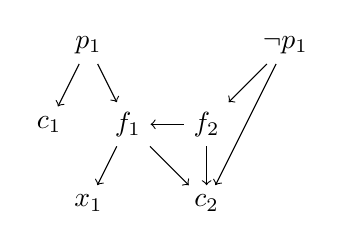
\begin{tikzpicture}[level distance=1cm,
    level 1/.style={sibling distance=3cm},
    level 2/.style={sibling distance=1.5cm}]
    
    \node (p) at (0.5, 0) {$p_1$};
    \node (np) at (3, 0) {$\lnot p_1$};
    \node (f) at (1, -1) {$f_1$};
    \node (g) at (2, -1) {$f_2$};
    \node (x) at (0.5, -2) {$x_1$};
    \node (c1) at (0, -1) {$c_1$};
    \node (c2) at (2, -2) {$c_2$};

    \path [->] (p) edge (f);
    \path [->] (p) edge (c1);

    \path [->] (np) edge (g);
    \path [->] (np) edge (c2);

    \path [->] (f) edge (x);
    \path [->] (f) edge (c2);

    \path [->] (g) edge (f);
    \path [->] (g) edge (c2);

  \end{tikzpicture}
\end{center}

Una struttura del genere è detta \textit{Prfectly Shared} (Perfettamente condivisa). Nella pratica questa
tecnica di condivisione di sottotermini è indispensabile dato che,
anche se a un costo per la creazione e la gestione non indifferente,
permette un risparmio di memoria e di tempo considerevole. Per effettuare ad esempio un controllo 
di uguaglianza tra due sottotermini è sufficiente controllare che le due frecce che partono dai termini padre
puntino allo stesso sottotermine, senza dover visitare l'intera sotto struttura, rendendo così tale operazione a tempo costante.


A questo punto definiamo finalmente le formule della logica del primo ordine. Prendendo come punto di partenza le formule proposizionali,
chiamiamo alfabeto delle formule del primo ordine 
$\Sigma' = \Sigma \cup \Sigma_f \cup \Sigma_p \cup \Sigma_x \cup \{\forall, \exists\}$ 
e definiamo come formule del primo ordine il linguaggio $F'$ generato dalla seguente grammatica:

$$ \phi := \top \mid \bot \mid A \mid \lnot \phi \mid (\phi \land \phi) \mid (\phi \lor \phi) \mid \forall x (\phi) \mid \exists x (\phi) $$

Dove $A$ è un atomo e $x$ è un simbolo di variabile. I simboli $\forall$ e $\exists$ sono detti quantificatori universali ed esistenziali.
Una variabile $x$ è detta \textit{vincolata} se è contenuta in una formula del tipo $\forall x (\varphi')$ o $\exists x (\varphi')$ 
altrimenti è detta \textit{libera}. Una formula è detta \textit{enunciato} se non contiene variabili libere. Una formula è detta 
\textit{ground} se tutti i suoi letterali sono ground.

Per comodità di scrittura è possibile raggruppare catene di quantificatori dello stesso tipo. Ad esempio, la formula 
$ \forall x_1 \forall x_2 \forall x_3 \exists x_4 \exists x_5 \forall x_6 \forall x_7 (\phi)$ può essere scritta come 
$\forall x_1 x_2 x_3 \exists x_4 x_5 \forall x_6 x_7 (\phi)$. Così come visto per $\lor$ e $\land$ è possibile vedere
$\forall$ e $\exists$ come operatori n-ari che prendono in input n-1 variabili e una formula.


% ---------------------- END Termini ----------------------

% ---------------------- Semantica ----------------------
\subsection{Semantica}


% ---------------------- END Semantica ----------------------

% ---------------------- Skolemizzazione e Forme Normali  ----------------------
\subsection{Skolemizzazione e Forme Normali}
In questo paragrafo verrà descritta una procedura fondamentale per la dimostrazione automatica di teoremi, la \textit{Skolemizzazione}. Varrà inoltre introdotta
una nuova forma normale chiamata \textit{PNF} e verranno
estese le forme normali descritte nel paragrafo della logica proposizionale per adattarle alla logica del primo ordine.


La definizione per le forme ENNF e NNF per la logica del primo ordine è pressoché identica a quella della logica proposizionale.
Come per la logica proposizionale, la trasformazione di una formula in ENNF/NNF preserva la relazione di conseguenza logica ed è sempre
possibile trasformare una formula in una equivalente in ENNF/NNF. 
Il calcolo per la normalizzazione viene effettuato allo stesso modo ma con l'aggiunta di due regole per la negazione dei quantificatori:

$$ \lnot \forall x (\varphi) \rightarrow \exists x (\lnot \varphi) $$
$$ \lnot \exists x (\varphi) \rightarrow \forall x (\lnot \varphi) $$


Chiameremo \textit{prefisso di quantificatori} una lista di quantificatori (es. $\forall x_1 \forall x_2 \exists x_3$). 
Un prefisso viene detto \textit{universale} se è composto esclusivamente da quantificatori universali e viene detto \textit{esistenziali} 
se è composto esclusivamente da quantificatori esistenziali. Una formula è in formato PNF (Prenex Normal Form) se tutti e soli 
i quantificatori si trovano all'inizio della formula. La classe di formule PNF è generata dalla seguente grammatica:

$$ P_0 := \rho(P) $$
$$ P := \top \mid \bot \mid A \mid \lnot P \mid (P \land P) \mid (P \lor P) $$

Dove $\rho$ è un prefisso di quantificatori e $A$ è un atomo.
La parte della formula generata dalla seconda regola viene spesso chiamata \textit{matrice}.
È sempre possibile normalizzare una formula in PNF, è un processo sound, ma non è sempre possibile mantenere la relazione di conseguenza logica.


La skolemizzazione è una procedura che permette di eliminare i quantificatori esistenziali da una formula. 
Sia $\rho$ un prefisso di quantificatori qualunque, la funzione $sk : F' \rightarrow F'$ può essere descritta in questo modo:

\begin{itemize}
  \item Se la formula è del tipo $\exists x(\rho \phi)$ allora $sk$ rimuove il primo quantificatore esistenziale e sostituisce 
  la variabile $x$ all'interno della formula con una nuova costante $c_{n+1}$, dove $n$ è il massimo indice di costante presente nella formula.

  \item Se la formula è del tipo $\forall x_k ... x_{k+m-1} \exists x_{k+m} (\rho \phi)$ allora $sk$ rimuove 
  il primo quantificatore esistenziale e sostituisce la variabile $x_{k+m}$ all'interno della formula con una nuova funzione 
  $f_{n+1}(x_k, ... , x_{k+m-1})$
  $m-1$-aria, dove $n$ è il massimo indice di funzione presente nella formula.
\end{itemize}

Applicando la funzione $sk$ tante volte quanto il numero di quantificatori esistenziali presenti nella formula si ottiene una formula 
senza quantificatori esistenziali. Anche la skolemizzazione è un processo sound, ma non è detto che preservi la conseguenza logica.



Combinando le tecniche apprese finora è possibile definire una procedura di normalizzazione che permette di trasformare una formula del primo ordine
in formato CNF. Le formule CNF per il primo ordine sono definite come segue:

$$ \zeta_0 := \rho(\zeta_1) $$
$$ \zeta_1 := \xi \mid (\xi \land \zeta_1) $$
$$ \xi := \top \mid \bot \mid C \mid \lnot C \mid (\xi \lor \xi ) $$

Dove $\rho$ è un prefisso di quantificatori universale. Per ottenere una formula CNF è sufficiente:

\begin{enumerate}
  \item Normalizzare la formula in NNF
  \item Normalizzare la formula in PNF
  \item Skolemizzare la formula
  \item Applicare lo stesso algoritmo di clausificazione descritto per la logica proposizionale sulla matrice della formula
\end{enumerate}

Visto le tecniche applicate il processo di clausificazione per la logica del primo ordine è sound ma non preserva la conseguenza logica.
Dato che in una formula CNF tutte le variabili sono universalmente quantificate per brevità è possibile omettere il prefisso di quantificatori.
Ad esempio, la formula CNF $\forall x_1 x_2 x_3 x_4 (\lnot p_1(x_1) \lor p_2(x_2) \lor p_3(x_3)) \land (\lnot p_4(x_4))$ può essere scritta come
$(\lnot p_1(x_1) \lor p_2(x_2) \lor p_3(x_3)) \land (\lnot p_4(x_4))$ e quindi rappresentata
in forma insiemistica come $\{\{\lnot p_1(x_1), p_2(x_2), p_3(x_3)\}, \{\lnot p_4(x_4)\}\}$.

% ---------------------- END Skolemizzazione e Forme Normali ----------------------


\subsection{Unificazione}

\section{Soddisfacibilità e Validità}
\section{Resolution}
\section{Il formato TPTP}

\end{document}